\newpage
\chapter{Software architecture}\SecLabel{SoftwareArchitecture}
 

\BornAgain\ is written on C++
and uses object oriented approach to 
achieve modularity, extensibility and transparency.
This leads to the task driven rather then command driven approach in 
different aspects  of the simulation and fitting of GISAS data.
User defines the sample structure, beam and detector characteristics,
fit parameters, using building
blocks -- \Code{classes} -- defined in core libraries of the framework.
These buildings blocks are combined together by the user according to his current
task using one the following approach.
\begin{itemize}
\item User creates a Python script with sample description and simulation settings
using \BornAgain\ API.
User runs the simulation by executing script in Python interpreter and then assess
simulation results using the way he likes, e.g. Python + numpy + matplotlib.
\item User may construct standalone C++ application linked to \BornAgain\ libraries.
\item User interacts with the framework through graphical 
user drag-and-drop interface (forthcoming).
\end{itemize}

Object oriented approach in the simulation design allows 
to reach much higher level of flexibility in sample construction, 
decouple interdependence in internal calculations and so facilitate creation of new models
that entails little or no modification to the existing code. 


\begin{figure}[htbp]
\centering
  \resizebox{0.9\textwidth}{!}{%
    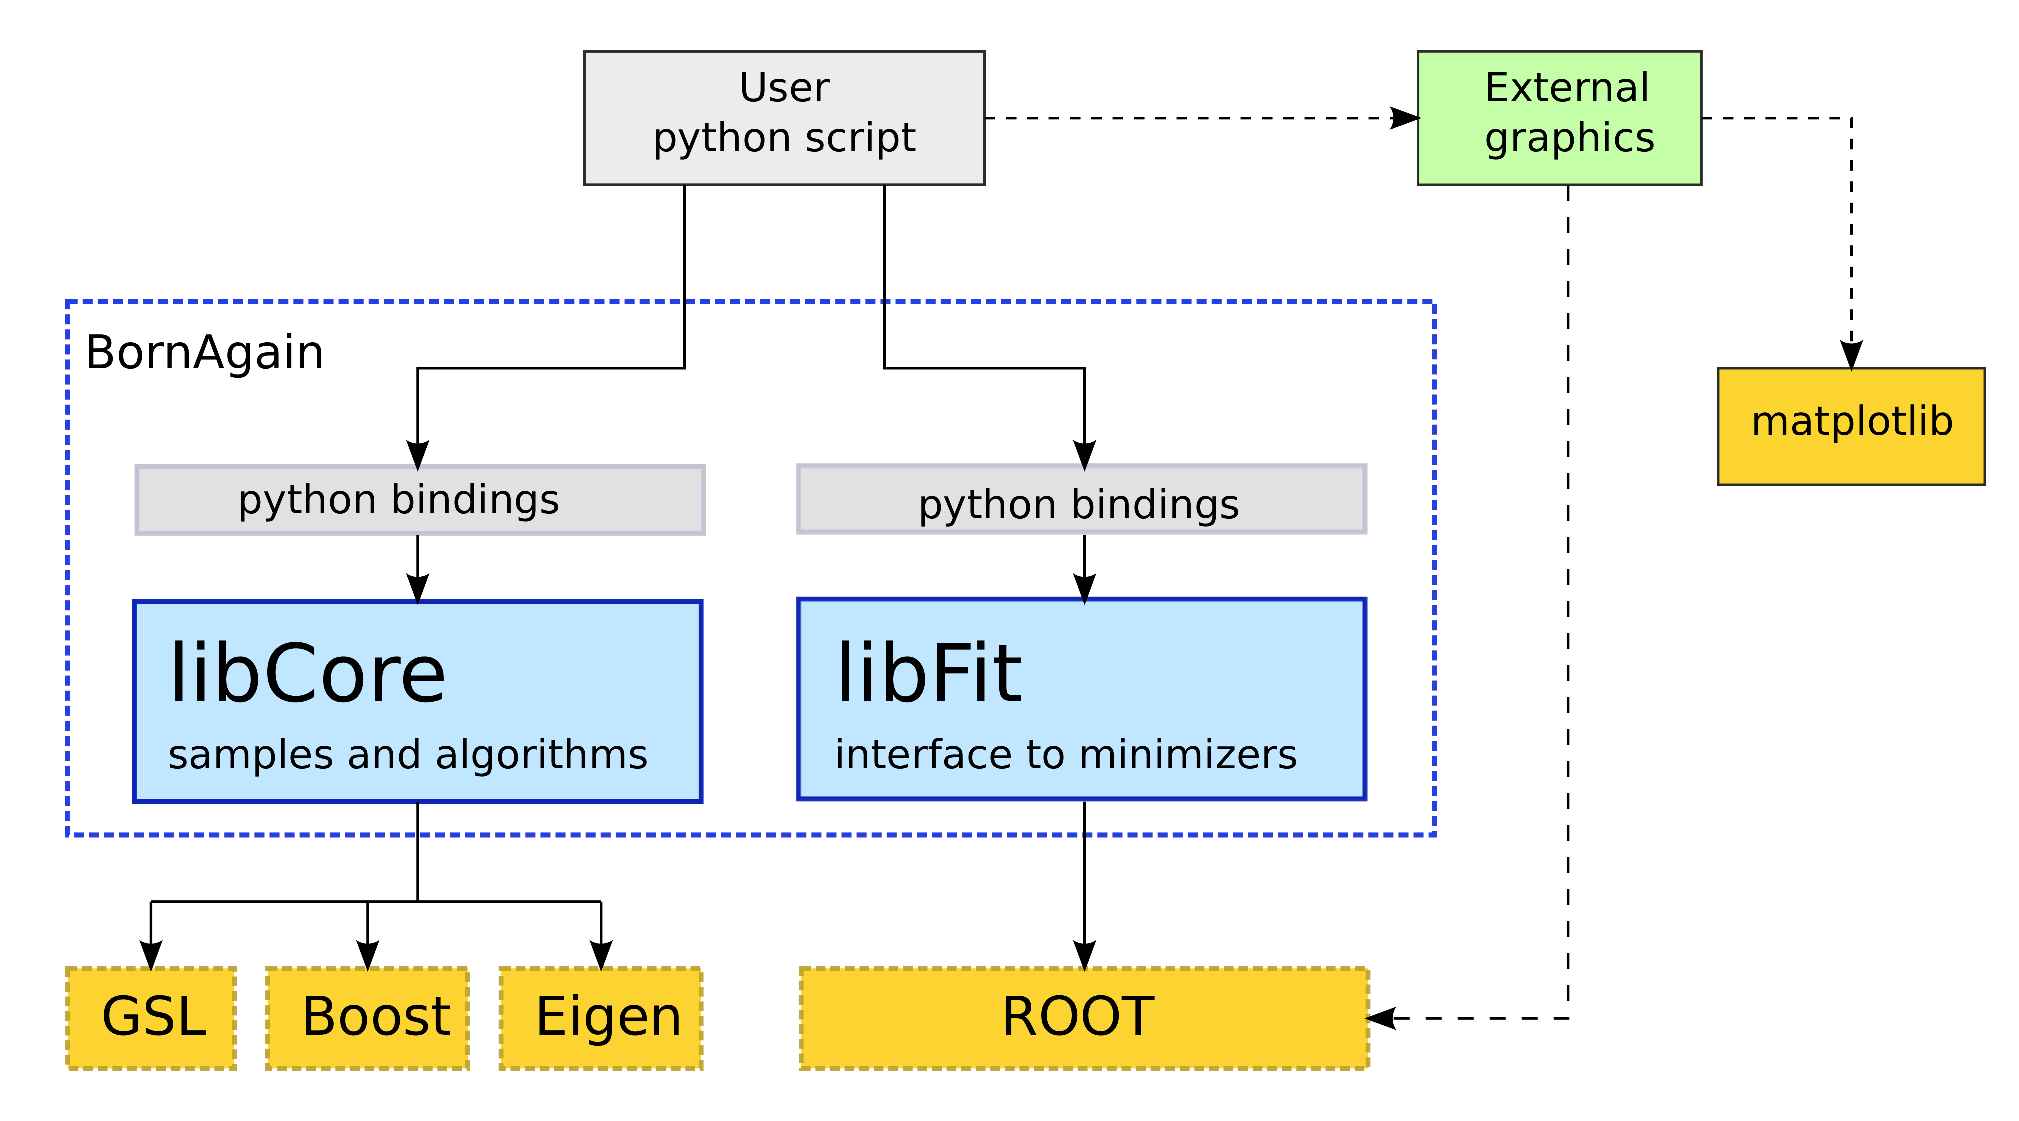
\includegraphics{Figures/basic_architecture.eps}}
\caption{
Structure of \BornAgain\ libraries.
}
\label{fig:two_ratios}
\end{figure}


The general structure of \BornAgain\ and the way the user interacts with it are
shown in Fig.~\ref{fig:two_ratios}.
The framework kernel consists of two shared libraries, \Code{libCore} and
\Code{libFit}. Thanks to the Python interface they can be imported to the Python as external modules. The library \Code{libCore} contains a number of classes, grouped into several class categories necessary for the description of model and running the simulation.
The library  \Code{libFit} contains a number of minimization engines 
and interfaces to them, to let user to fit real data with the model defined.

\BornAgain\ depends from a few external well established open-source libraries: boost, GNU scientific library, Eigen and Fast Fourier Transformation libraries. They are required to be present on the system to run \BornAgain\ on Unix Platform. In the case of Windows Platform they will be added to the system automatically with \BornAgain\ installation. Other libraries shown
on the plot (ROOT, matplotlib) are optional.

 


%\section{Design overview}

% general considerations
% general capabilities and properties
% openess 
% global structure
% design and architecture

% Software process
% - configuration and release management
% - quality assurance and testing
% - user support process


% The BornAgain framework provides a number of classes, grouped into several class categories.

